\section*{Exposé}
\label{sec:abstract}

Die Interaktion eines Nutzers mit dem Endgerät wie Smartphone oder PC ist sehr vielfältig und schwierig vorherzusagen. Dennoch lassen sich womöglich Nutzer-spezifische (also personalisierte) als auch globale (kollaborative) Muster mit Hilfe der vorausgehenden Nutzerinteraktionen herausarbeiten. Diese könnten dazu verwendet werden die Absicht eines Nutzers oder einer Nutzergruppe vorauszusagen. Dabei ist es interessant zu wissen bis zu welchem Detailgrad diese Vorhersagen zuverlässig getroffen werden können.

Es bietet sich an, dies mit Hilfe der Nutzerinteraktionen in Sessions auf Android Geräten umzusetzten. Dazu könnten die Sequentiellen UI Tree Daten des Gerätes verfolgt, gefiltert und gelabelt werden und anschließend mit einem Machine-Learning-Modell so trainiert werden, ähnliche Interaktions-Sequenzen zu finden und Vorhersagen zu treffen. Diese können dann sehr grob sein, z.B. durch Vorhersage der nächsten App. Oder sie können sehr detailliert sein, z.B. die Bestimmung der nächsten Nutzeraktion, wie das Ausfüllen eines Formularfeldes.

Es soll ein Konzept erarbeitet werden, wie ein Modell für die Vorhersage der Nutzerabsicht aufgebaut sein könnte und wie dieses für den Nutzer angewendet werden könnte. Dazu werden Möglichkeiten für die Sammlung und Vektorisierung von sequentiellen UI Trees (z.B. des Android Accessibility Service) erörtert (z.B. via Recurrent Neural Network (\textit{RNN}) \cite{quadrana2017personalizing} \cite{bansal2022remembering} \cite{pietro2022recommendationSystems}, \textit{Seq2Seq} Modell \cite{chollet2017seq2seq}, \textit{Intention2Text} \cite{yu2020understanding}, \textit{Html2Vec} \cite{wu2022distributed}), die der Vorhersage des Nutzerintents dienen sollen. Dabei spielt der Datenschutz und die Vorfilterung der Features in den UI Daten eine wichtige Rolle. Danach können personalisierte als auch kollaborative Daten bei einem hybriden Ansatz Verwendung finden. Dieses Modell soll dann in einem Android-App-Service dem Nutzer bereit gestellt werden und diesem je nach Detail-Grad kommende Apps oder Aktionen zu einem passendem Zeitpunkt vorschlagen. Dabei ist auch zu berücksichtigen, ob der Nutzer beim Lernprozess beitragen kann und vorgeschlagene Aktionen durch Feedback (Labeling) verbessert.
Die Performance des Modells kann beispielsweise anhand von Indikatoren wie der Menge an Trainingsdaten und zeitlicher Aufwand des Lernprozesses gemessen werden. Die Wirksamkeit kann durch Genauigkeitsmetriken bei der Vorhersage von beispielsweise App-Kategorien \cite{google2023appCategory} oder kompletten Testsequenzen via Rico \cite{deka2017rico} oder ERICA \cite{deka2016erica} evaluiert werden.

Ferner könnte das Machine-Learning-Modell neben der Intent-Prediction folgende Vorteile bieten:
\begin{itemize}
  \item Reduzierung der Komplexität und Größe des UI Trees
  \item Erstellung von Nutzergruppen, die ein ähnliches Verhalten bei der Nutzung digitaler UI-Systeme haben
  \item Wegfall von technischem Know-How zu einzelnen Features, das für einen manuellen Vergleich von Nutzer-Sessions nötig wäre \cite{ghods2019activity2vec}
  \item Berücksichtigung des zeitlichen Verlaufs eines Nutzers (sequentiell)
  \item Vergleich von Nutzerinteraktionen ohne in die Privatsphäre eingreifende Informationen
  \item Unterstützung von App-Entwicklern zur Verbesserung des Designs und der Usability
  \item Anwendung in Psychologie und Marktforschung
\end{itemize}

\begin{figure}
  \centering
  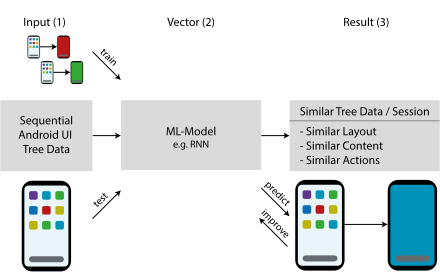
\includegraphics[width=\textwidth]{vectorization.svg}
  \caption{Possible procedure using a Machine-Learning algorithm to predict the next intent from a beginning user session: The input (1) can be a sequence of Android tree data. With help of a Machine-Learning-Model (2) (e.g. RNN) a vector representation can be trained and then predict the most probable action or screen (3) from a given starting sequence.}
  \label{fig:encode-decode}
\end{figure}

\begin{figure}
  \centering
  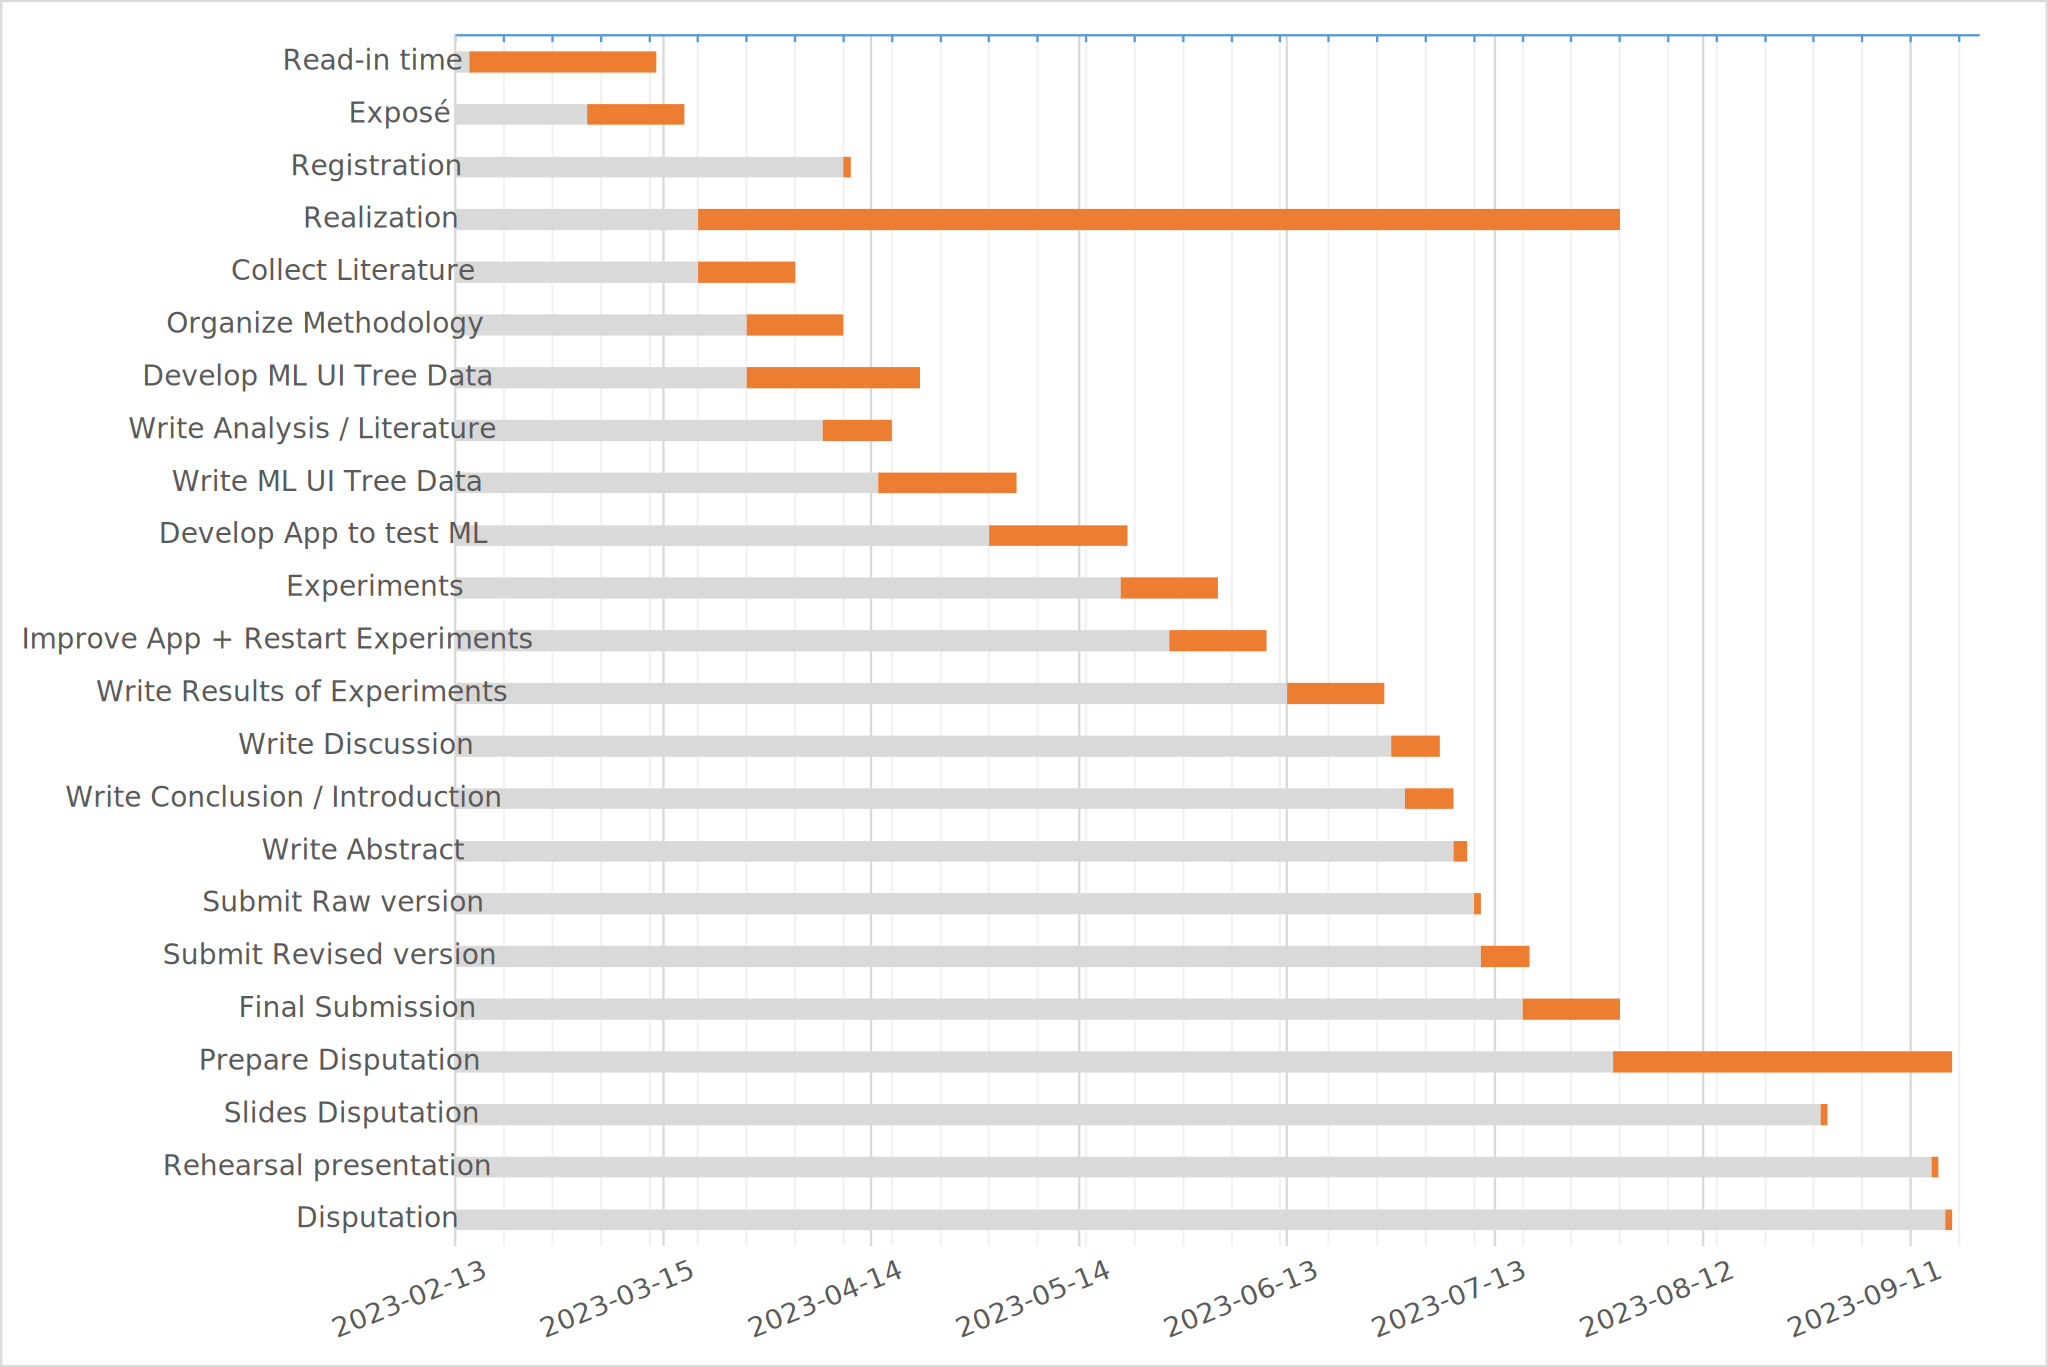
\includegraphics[width=\textwidth]{graphics/TimeTable-Gantt.svg}
  \caption{Schedule as a Gantt Chart}
  \label{fig:schedule}
\end{figure}